\documentclass[12pt, twoside]{article}
\usepackage[francais]{babel}
\usepackage[T1]{fontenc}
\usepackage[latin1]{inputenc}
\usepackage[left=5mm, right=5mm, top=6mm, bottom=6mm]{geometry}
\usepackage{float}
\usepackage{graphicx}
\usepackage{array}
\usepackage{multirow}
\usepackage{amsmath,amssymb,mathrsfs}
\usepackage{soul}
\usepackage{textcomp}
\usepackage{eurosym}
 \usepackage{variations}
\usepackage{tabvar}


\pagestyle{empty}

\begin{document}


\section*{\center{Devoir maison 9}}


\bigskip


\textit{Devoir � rendre sur feuille grand format pour le \ul{mercredi 29 mai
2013}. Chaque r�ponse sera justifi�e.}

\bigskip

\bigskip

\ul{Exercice 1}: \textit{2 points}

\begin{tabular}{cc}
\begin{minipage}{10cm}
Calculer EF. Justifier votre r�ponse.
\end{minipage}
&
\begin{minipage}{8cm}
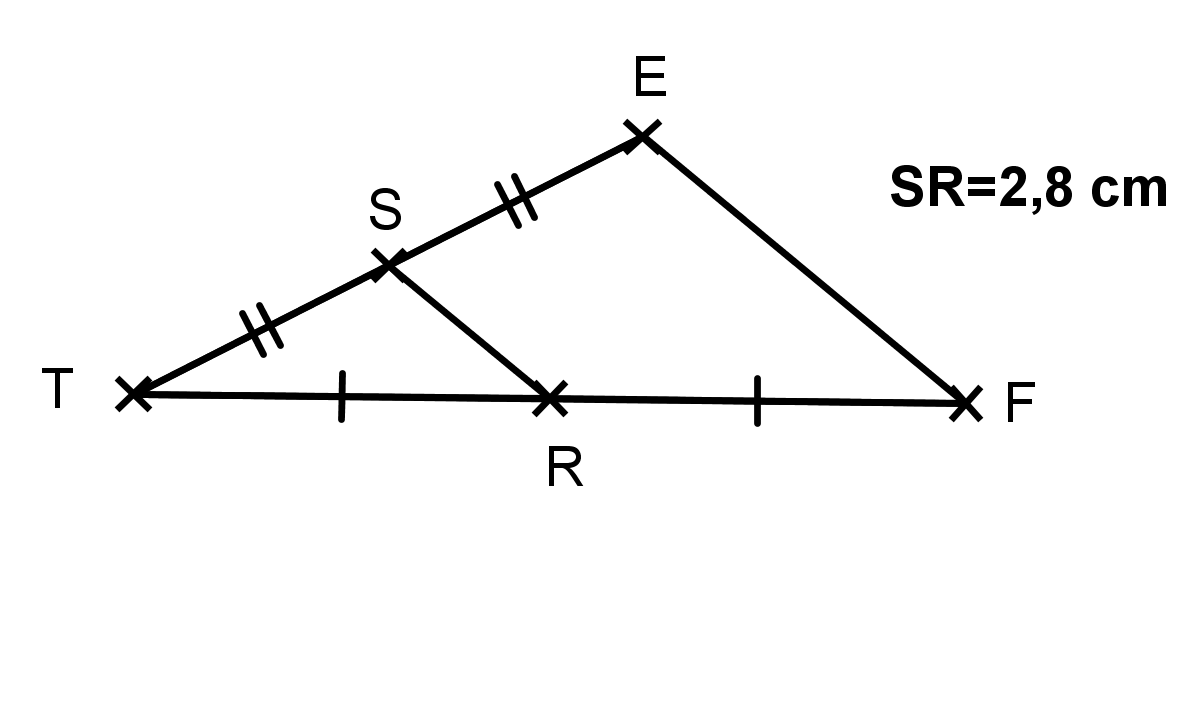
\includegraphics[width=5cm]{images/ex1.png}
\end{minipage}
\end{tabular}

\bigskip


\bigskip

\ul{Exercice 2}: \textit{6 points}

\begin{enumerate}
  \item GAZ est un triangle rectangle en A. Les points F, E et R sont les
  milieux respectifs de [AZ], [GZ] et [GA]. Faire une figure.
  \item 
  
  \begin{enumerate}
    \item D�montrer que les droites (RE) et (AZ) sont parall�les.
    \item D�montrer que les droites (AG) et (EF) sont parall�les.
    \item Montrer que FERA est un rectangle. Justifer votre r�ponse (on pourra
    commencer par montrer que FERA est un parall�logramme).
\end{enumerate}
\end{enumerate}

\bigskip


\bigskip


\ul{\textbf{Exercice 3}}: \textit{4,5 points}

Dans la figure ci-dessous, le point A appartient au cercle de diam�tre [CT] et
de centre S. Les droites (HS) et (CA) sont perpendiculaires.


\begin{tabular}{cc}
\begin{minipage}{13cm}
\begin{enumerate}
  \item D�monter que les droites (CA) et (AT) sont perpendiculaires.
  \item En d�duire que les droites (HS) et (AT) sont parall�les. Justifier
  votre r�ponse.
  \item D�montrer que H est le milieu du segment [CA].
\end{enumerate}
\end{minipage}
&
\begin{minipage}{5cm}
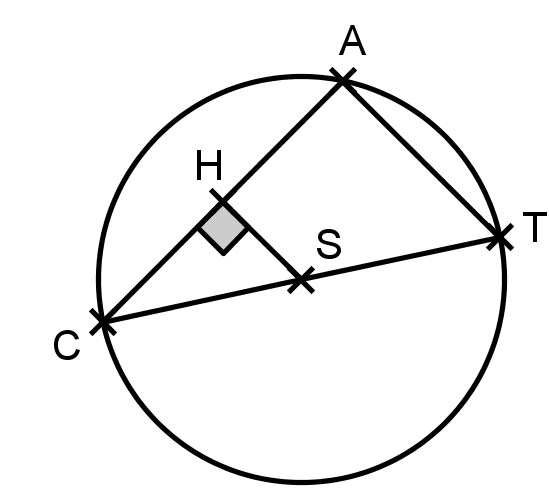
\includegraphics[width=4cm]{images/ex4.png}
\end{minipage}
\end{tabular}


\bigskip

\bigskip


\ul{Exercice 4}: (\textit{3,5 points})

\enskip

On a relev� la nationalit� des vainqueurs de 97 tours de France de cyclisme
entre 1903 et 2010. Le tableau ci-dessous donne les nationalit�s des vainqueurs
et la fr�quence de victoires.

\begin{center}
\begin{tabular}{|c|c|c|c|c|c|}
\hline
Pays & France & Belgique & Espagne & Etats-Unis & Autres \\

\hline

Nombre de victoires & 36 & 18 & 13 & 10 & 20 \\

\hline

fr�quence en \% & \ldots \ldots & 18,6 & 13,4 & 10,3 & 20,6 \\

\hline
\end{tabular}
\end{center}


\begin{enumerate}
  \item Calculer la fr�quence en pourcentage de victoires fran�aises, arrondie
  � 0,1\% pr�s.
  \item On veut r�aliser un diagramme circulaire repr�sentant la r�partition
  des nationalit�s des vainqueurs.
  
  \begin{enumerate}
    \item Calculer les mesures d'angles repr�sentant les victoires de chaque
    pays, arrondie au degr� pr�s. On pourra faire un tableau de
    proportionnalit�.
    \item Construire ce diagramme circulaire.
  \end{enumerate}
  
\end{enumerate}


\bigskip

\bigskip

\ul{Exercice 5}: (\textit{2 points})


\enskip

Un serveur dans un bar  fait le bilan des pourboires qu'il a gagn�s chaque
jour. Calculer la moyenne journali�re de ses pourboires.


\begin{center}
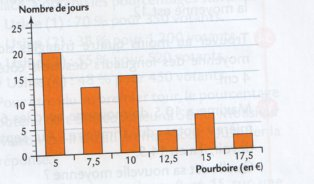
\includegraphics[width=9cm]{images/ex4.jpg}
\end{center}


\bigskip

\bigskip

\ul{Exercice 6 }: (\textit{2 points})

\enskip

Dans une salle de concert, le niveau sonore est affich� toutes les minutes.
Voici les relev�s (en d�cibels) au cours d'une demi-heure:

\begin{center}
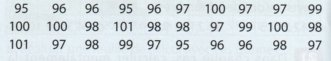
\includegraphics[width=7cm]{images/ex6.jpg}
\end{center}


\begin{enumerate}
  \item Pr�senter ces donn�es dans un tableau d'effectifs.
  \item Calculer le niveau sonore moyen.
\end{enumerate}

\end{document}
